% ===================================================================
%  Week 2 — Session 2: Thresholding & Advanced Enhancement
%  Compile: pdflatex -interaction=nonstopmode slides-b.tex  (twice)
% ===================================================================
\documentclass[10pt,aspectratio=169]{beamer}
% ===================================================================
%  Shared Beamer preamble for "Practical Image Processing"
%  English slides. Compile with pdfLaTeX.
% ===================================================================

\usetheme{metropolis}
\usepackage[T1]{fontenc}
\usepackage[utf8]{inputenc}
\usepackage{lmodern}
\usepackage{listings}
\usepackage{tcolorbox}
\usepackage{fontawesome5}
\usepackage{booktabs}
\usepackage{amsmath,amssymb}
\usepackage{tikz}
\usepackage{pgfplots}
\pgfplotsset{compat=1.17}
\usetikzlibrary{arrows.meta,positioning,shapes.geometric,fit,backgrounds,matrix}
\tcbuselibrary{skins,breakable}

% ---- Palette --------------------------------------------------------
\definecolor{coursePrimary}{HTML}{1B4965}   % deep blue
\definecolor{courseAccent}{HTML}{E76F51}    % coral
\definecolor{courseGood}{HTML}{2A9D8F}      % teal
\definecolor{courseBad}{HTML}{C0392B}       % red
\definecolor{courseInfo}{HTML}{2980B9}      % blue
\definecolor{codeBg}{HTML}{F5F6FA}
\definecolor{codeKw}{HTML}{8E44AD}
\definecolor{codeStr}{HTML}{2A9D8F}
\definecolor{codeCom}{HTML}{7F8C8D}

\setbeamercolor{frametitle}{bg=coursePrimary}
\setbeamercolor{progress bar}{fg=courseAccent}
\setbeamercolor{alerted text}{fg=courseAccent}
\metroset{block=fill,sectionpage=progressbar,numbering=fraction}

% ---- Code listings (Python is built into listings) -----------------
\lstdefinestyle{course}{
  backgroundcolor=\color{codeBg},
  basicstyle=\ttfamily\scriptsize,
  keywordstyle=\color{codeKw}\bfseries,
  stringstyle=\color{codeStr},
  commentstyle=\color{codeCom}\itshape,
  numberstyle=\tiny\color{codeCom},
  numbers=left, numbersep=6pt,
  showstringspaces=false, breaklines=true, breakatwhitespace=true,
  tabsize=4, columns=fullflexible,
  frame=single, framesep=4pt, rulecolor=\color{gray!30},
  keepspaces=true, upquote=true, language=Python,
}
\lstset{style=course}
\lstdefinelanguage{bash}{
  keywords={cd,pip,python,venv,source,import}, sensitive=true,
  morecomment=[l]{\#}, morestring=[b]', morestring=[b]",
}

% ---- Reusable callout boxes ----------------------------------------
\newtcolorbox{goodbox}[1][Good practice]{colback=courseGood!8,colframe=courseGood,
  fonttitle=\bfseries,title={\faCheck~#1},boxrule=0.6pt,left=4pt,right=4pt,top=3pt,bottom=3pt}
\newtcolorbox{badbox}[1][Pitfall]{colback=courseBad!8,colframe=courseBad,
  fonttitle=\bfseries,title={\faTimes~#1},boxrule=0.6pt,left=4pt,right=4pt,top=3pt,bottom=3pt}
\newtcolorbox{infobox}[1][Note]{colback=courseInfo!8,colframe=courseInfo,
  fonttitle=\bfseries,title={\faInfoCircle~#1},boxrule=0.6pt,left=4pt,right=4pt,top=3pt,bottom=3pt}
\newtcolorbox{mathbox}[1][Math]{colback=coursePrimary!6,colframe=coursePrimary,
  fonttitle=\bfseries,title={\faCalculator~#1},boxrule=0.6pt,left=4pt,right=4pt,top=3pt,bottom=3pt}

\newcommand{\keyidea}[1]{\begin{alertblock}{Key idea}#1\end{alertblock}}
\newcommand{\term}[1]{\textbf{\color{coursePrimary}#1}}
\newcommand{\code}[1]{\lstinline[basicstyle=\ttfamily\small]|#1|}

% ---- A helper to draw a small pixel grid, cells shaded by value ----
% \pixelgrid{ {10,20,120,200,240}, {30,60,130,180,230}, ... }
\newcommand{\pixelgrid}[1]{%
  \begin{tikzpicture}[font=\scriptsize,scale=0.6]
    \foreach \row [count=\ry] in {#1} {
      \foreach \val [count=\cx] in \row {
        \draw[gray,fill=coursePrimary!8] (\cx,-\ry) rectangle ++(1,-1);
        \node at (\cx+0.5,-\ry-0.5) {\val};
      }
    }
  \end{tikzpicture}}


\title{Point Operations \& Histograms}
\subtitle{Week 2 — Session 2: Thresholding \& advanced enhancement}
\author{Practical Image Processing}
\date{Lecture 2.2 \textbullet\ 60--70 min}

\begin{document}

\maketitle

\begin{frame}{Recap of Session 1}
  \begin{columns}[T]
    \begin{column}{0.58\textwidth}
      \begin{itemize}
        \item The \term{histogram} diagnoses exposure/contrast \emph{before} you touch a pixel.
        \item \term{Point operations} $s=T(r)$: brightness, contrast, negative, gamma — all a LUT.
        \item \term{Stretch} and \term{equalization} spread a bunched histogram across 0--255.
        \item \alert{Today:} turn those enhanced grays into a clean \term{binary mask}, then go deeper
              (CLAHE, matching, color).
      \end{itemize}
    \end{column}
    \begin{column}{0.42\textwidth}
      \begin{alertblock}{The goal}
        DocScan needs the meter digits as a crisp black-on-white mask for the next stages.
      \end{alertblock}
    \end{column}
  \end{columns}
\end{frame}

\begin{frame}{Roadmap}\tableofcontents\end{frame}

% ==================================================================
\section{Thresholding}
% ==================================================================

\begin{frame}{Thresholding: intensity $\rightarrow$ two classes}
  \begin{columns}[T]
    \begin{column}{0.5\textwidth}
      \begin{center}
      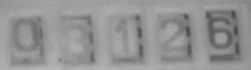
\includegraphics[width=0.9\linewidth]{../assets/gray.png}\\{\scriptsize grayscale meter}\\[4pt]
      
\includegraphics[width=0.9\linewidth]{../assets/otsu.png}\\{\scriptsize Otsu binary: digits vs background}
      \end{center}
    \end{column}
    \begin{column}{0.5\textwidth}
      \begin{itemize}
        \item $s = 255$ if $r>T$ else $0$. Turns gray into black/white.
        \item The whole game is choosing $T$. A bimodal histogram makes it easy.
        \item This is DocScan's ``make it crisp'' step — digits become a clean mask.
      \end{itemize}
    \end{column}
  \end{columns}
\end{frame}

\begin{frame}{Threshold as a transfer function}
  \begin{columns}[T]
    \begin{column}{0.55\textwidth}
    \begin{center}
    \begin{tikzpicture}
      \begin{axis}[width=6cm,height=4.4cm,xmin=0,xmax=255,ymin=-15,ymax=270,font=\tiny,
        xlabel={input $r$},ylabel={output $s$},xtick={0,128,255},ytick={0,255}]
        \addplot[coursePrimary,thick] coordinates{(0,0)(128,0)};
        \addplot[coursePrimary,thick] coordinates{(128,255)(255,255)};
        \addplot[courseBad,dashed] coordinates{(128,-15)(128,270)};
        \node[font=\tiny,courseBad] at (axis cs:150,130) {$T$};
      \end{axis}
    \end{tikzpicture}
    \end{center}
    \end{column}
    \begin{column}{0.45\textwidth}
      \begin{itemize}
        \item A \term{step} at $T$: the most extreme point operation.
        \item Everything below $T$ collapses to one class, everything above to the other.
        \item All the subtlety moves into \emph{where} to put the step.
      \end{itemize}
    \end{column}
  \end{columns}
\end{frame}

\begin{frame}{Choosing $T$ from a bimodal histogram}
  \begin{center}
  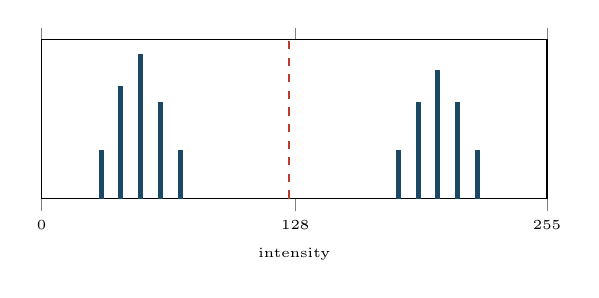
\begin{tikzpicture}
    \begin{axis}[width=8cm,height=3.6cm,ybar,bar width=1.4pt,ymin=0,xmin=0,xmax=255,
      xtick={0,128,255},ytick=\empty,font=\tiny,xlabel={intensity}]
      \addplot[draw=coursePrimary,fill=coursePrimary]
        coordinates{(30,3)(40,7)(50,9)(60,6)(70,3)(180,3)(190,6)(200,8)(210,6)(220,3)};
      \draw[courseBad,thick,dashed] (axis cs:125,0) -- (axis cs:125,10);
      \node[courseBad,font=\tiny] at (axis cs:125,10.8) {$T$};
    \end{axis}
  \end{tikzpicture}
  \end{center}
  \begin{itemize}
    \item Two humps = object vs background. The \term{valley} between them is the natural $T$.
    \item Put $T$ in the valley $\rightarrow$ few pixels are misclassified.
    \item But eyeballing the valley doesn't scale — we want it \emph{automatic}.
  \end{itemize}
\end{frame}

\begin{frame}{Otsu: pick the threshold automatically}
  \begin{itemize}
    \item Otsu's method finds the $T$ that best \term{separates} the two histogram humps.
    \item Formally: minimize the within-class variance (equivalently, maximize between-class variance).
    \item One line: \code{cv2.threshold(g, 0, 255, THRESH\_BINARY+THRESH\_OTSU)}.
  \end{itemize}
  \begin{mathbox}
    Between-class variance at threshold $T$:
    $\sigma_b^2(T) = \omega_0(T)\,\omega_1(T)\,\big[\mu_0(T)-\mu_1(T)\big]^2$,
    where $\omega_i$ are class weights and $\mu_i$ class means. Otsu picks $T^\star=\arg\max_T \sigma_b^2(T)$.
  \end{mathbox}
\end{frame}

\begin{frame}{Why maximize between-class variance?}
  \begin{itemize}
    \item Total variance $\sigma^2 = \sigma_w^2(T) + \sigma_b^2(T)$ is \emph{constant} (doesn't depend on $T$).
    \item So minimizing \term{within}-class spread $\equiv$ maximizing \term{between}-class separation.
    \item Between-class is cheap: just class weights $\omega_i$ and means $\mu_i$, both from the histogram.
    \item Sweep $T=0\ldots255$, evaluate $\sigma_b^2(T)$, keep the best — a 256-step loop.
  \end{itemize}
  \begin{goodbox}
    Otsu needs \emph{no parameters} and runs on the histogram alone — perfect for a bimodal meter crop.
  \end{goodbox}
\end{frame}

\begin{frame}{Worked example: Otsu on two classes}
  \begin{mathbox}
    3 dark pixels at $\{40,50,60\}$ and 3 bright at $\{200,210,220\}$; try $T=125$.
  \end{mathbox}
  \begin{itemize}
    \item Weights: $\omega_0=\tfrac{3}{6}=0.5$, $\omega_1=0.5$.
    \item Means: $\mu_0=\tfrac{40+50+60}{3}=50$, $\mu_1=\tfrac{200+210+220}{3}=210$.
    \item $\sigma_b^2 = 0.5\cdot0.5\cdot(50-210)^2 = 0.25\cdot 25600 = 6400$ — large \& maximal, since any other $T$
          moves a pixel to the ``wrong'' class and shrinks $(\mu_0-\mu_1)^2$.
  \end{itemize}
  \keyidea{The best split sits in the empty valley — exactly where the two means are farthest apart.}
\end{frame}

\begin{frame}[fragile]{Otsu in code (and reading the result)}
\begin{lstlisting}[language=Python]
T, binary = cv2.threshold(gray, 0, 255,
                          cv2.THRESH_BINARY + cv2.THRESH_OTSU)
print('Otsu chose T =', T)          # the automatic threshold
# invert if digits came out white-on-black:
# binary = cv2.bitwise_not(binary)
\end{lstlisting}
  \begin{infobox}
    Pass \code{0} as the threshold arg — the \code{OTSU} flag tells OpenCV to compute $T$ for you and return it.
  \end{infobox}
\end{frame}

\begin{frame}{When a single global $T$ fails}
  \begin{columns}[T]
    \begin{column}{0.5\textwidth}
      \begin{center}
      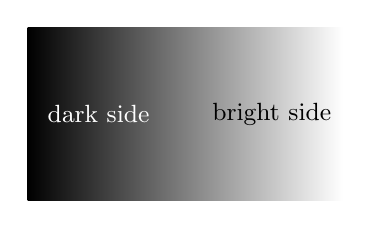
\begin{tikzpicture}
        \shade[left color=black,right color=white] (0,0) rectangle (4,2.2);
        \node[white] at (0.9,1.1) {\small dark side};
        \node[black] at (3.1,1.1) {\small bright side};
      \end{tikzpicture}\\{\scriptsize a shadow gradient across the page}
      \end{center}
    \end{column}
    \begin{column}{0.5\textwidth}
      \begin{badbox}
        Otsu assumes two clear classes with even lighting. Under a shadow gradient, one global $T$
        blackens the dark side and whitens the bright side — digits vanish on both.
      \end{badbox}
    \end{column}
  \end{columns}
\end{frame}

% ==================================================================
\section{Adaptive thresholding}
% ==================================================================

\begin{frame}{Adaptive thresholding: a local $T$ per neighbourhood}
  \begin{columns}[T]
    \begin{column}{0.5\textwidth}
    \begin{center}
    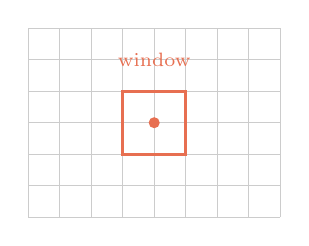
\begin{tikzpicture}[font=\scriptsize]
      \draw[step=0.4,gray!40] (0,0) grid (3.2,2.4);
      \draw[courseAccent,very thick] (1.2,0.8) rectangle (2.0,1.6);
      \fill[courseAccent] (1.6,1.2) circle (2pt);
      \node[courseAccent] at (1.6,2.0) {window};
    \end{tikzpicture}\\{\scriptsize $T$ = local mean $-\,C$, computed per pixel}
    \end{center}
    \end{column}
    \begin{column}{0.5\textwidth}
      \begin{itemize}
        \item Slide a window; threshold each pixel against \term{its own} neighbourhood.
        \item Local mean (or Gaussian-weighted mean) tracks the lighting gradient.
        \item Subtract a constant $C$ to bias against noise in flat regions.
      \end{itemize}
    \end{column}
  \end{columns}
\end{frame}

\begin{frame}[fragile]{Adaptive thresholding for uneven light}
\begin{lstlisting}[language=Python]
# a local threshold per neighbourhood -> robust to shadows/gradients
binary = cv2.adaptiveThreshold(gray, 255, cv2.ADAPTIVE_THRESH_GAUSSIAN_C,
                               cv2.THRESH_BINARY, blockSize=31, C=10)
\end{lstlisting}
  \keyidea{Global Otsu for even lighting; adaptive for real photos with shadows. DocScan photos usually need adaptive.}
\end{frame}

\begin{frame}{Tuning blockSize and C}
  \begin{itemize}
    \item \code{blockSize} = neighbourhood size (odd). Too small $\rightarrow$ speckle; too large $\rightarrow$ acts global again.
    \item \code{C} = margin subtracted from the local mean. Larger $C$ $\rightarrow$ fewer white pixels (kills noise, may thin digits).
    \item Rule of thumb: \code{blockSize} a bit larger than the stroke width you want to keep.
  \end{itemize}
  \begin{columns}[T]
    \begin{column}{0.5\textwidth}
      \begin{badbox}
        \code{blockSize} too small turns texture/noise into a confetti of speckles.
      \end{badbox}
    \end{column}
    \begin{column}{0.5\textwidth}
      \begin{goodbox}
        Enhance first (gamma/CLAHE), \emph{then} threshold — a cleaner input makes tuning far easier.
      \end{goodbox}
    \end{column}
  \end{columns}
\end{frame}

% ==================================================================
\section{Advanced enhancement}
% ==================================================================

\begin{frame}{CLAHE: local, limited equalization}
  \begin{itemize}
    \item Global equalization over-amplifies noise in flat regions.
    \item \term{CLAHE} equalizes in small tiles and \term{clips} the histogram to limit amplification.
    \item Usually the better default for real photos: \code{cv2.createCLAHE(clipLimit=2.0)}.
  \end{itemize}
  \begin{goodbox}
    For DocScan, CLAHE on the value channel often beats plain equalization — local contrast without the noise blow-up.
  \end{goodbox}
\end{frame}

\begin{frame}{How CLAHE works}
  \begin{columns}[T]
    \begin{column}{0.5\textwidth}
    \begin{center}
    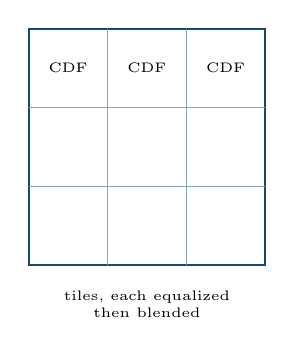
\begin{tikzpicture}[font=\scriptsize]
      \draw[coursePrimary,thick] (0,0) rectangle (3,3);
      \foreach \x in {1,2} \draw[coursePrimary!50] (\x,0)--(\x,3);
      \foreach \y in {1,2} \draw[coursePrimary!50] (0,\y)--(3,\y);
      \node at (0.5,2.5){\tiny CDF};\node at (1.5,2.5){\tiny CDF};\node at (2.5,2.5){\tiny CDF};
      \node[align=center] at (1.5,-0.5){\tiny tiles, each equalized\\[-2pt]\tiny then blended};
    \end{tikzpicture}
    \end{center}
    \end{column}
    \begin{column}{0.5\textwidth}
      \begin{enumerate}
        \item Split the image into a grid of \term{tiles}.
        \item Build each tile's histogram; \term{clip} bars above \code{clipLimit}, redistribute the excess.
        \item Equalize each tile; \term{bilinearly interpolate} between tile maps to avoid seams.
      \end{enumerate}
    \end{column}
  \end{columns}
\end{frame}

\begin{frame}[fragile]{CLAHE in code}
\begin{lstlisting}[language=Python]
clahe = cv2.createCLAHE(clipLimit=2.0, tileGridSize=(8, 8))
out = clahe.apply(gray)              # local contrast, noise held down
\end{lstlisting}
  \begin{itemize}
    \item \code{clipLimit}: higher = stronger local contrast (and more noise). 2--3 is a safe start.
    \item \code{tileGridSize}: more tiles = more local, but risk of blotchiness on smooth areas.
  \end{itemize}
  \begin{infobox}
    CLAHE is deterministic given its parameters — good for a repeatable pipeline.
  \end{infobox}
\end{frame}

\begin{frame}{Why equalization can hurt}
  \begin{itemize}
    \item It's data-driven and \term{unpredictable}: two similar images can map very differently.
    \item It amplifies whatever is there — including sensor noise and JPEG blocks.
    \item For a pipeline, prefer a \term{deterministic} op (fixed gamma/stretch) so later stages are stable.
  \end{itemize}
  \keyidea{``Looks better to the eye'' $\ne$ ``better for the next algorithm.'' Enhance for the goal, not the demo.}
\end{frame}

\begin{frame}{Histogram matching}
  \begin{columns}[T]
    \begin{column}{0.55\textwidth}
      \begin{itemize}
        \item Sometimes you want an image's histogram to \emph{match} a reference (consistent look across a dataset).
        \item Useful when meter photos come from many cameras/lightings and you want uniform input.
        \item Map via the two CDFs — the same machinery as equalization, but to a target shape.
      \end{itemize}
    \end{column}
    \begin{column}{0.45\textwidth}
    \begin{center}
    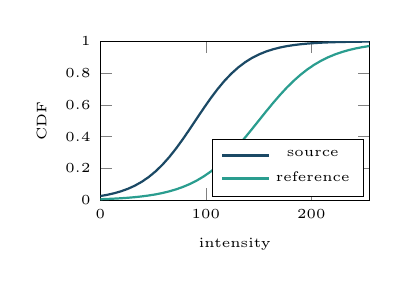
\begin{tikzpicture}
      \begin{axis}[width=5cm,height=3.6cm,xmin=0,xmax=255,ymin=0,ymax=1,font=\tiny,
        xlabel={intensity},ylabel={CDF},samples=40,
        legend style={font=\tiny,at={(0.98,0.02)},anchor=south east}]
        \addplot[coursePrimary,thick,domain=0:255]{1/(1+exp(-(x-90)/25))};\addlegendentry{source}
        \addplot[courseGood,thick,domain=0:255]{1/(1+exp(-(x-150)/30))};\addlegendentry{reference}
      \end{axis}
    \end{tikzpicture}
    \end{center}
    \end{column}
  \end{columns}
  \begin{mathbox}
    For each $r$: find $z$ with $\mathrm{CDF}_{\text{ref}}(z)=\mathrm{CDF}_{\text{src}}(r)$, then map $r\mapsto z$.
  \end{mathbox}
\end{frame}

% ==================================================================
\section{Color}
% ==================================================================

\begin{frame}{Color: enhance value, not each channel}
  \begin{itemize}
    \item Equalizing R, G, B \emph{separately} shifts colors (ugly casts).
    \item Convert to HSV/Lab, enhance the \term{value/lightness} channel, convert back.
    \item Keeps hue intact while fixing brightness/contrast — the correct way to enhance color photos.
  \end{itemize}
  \begin{badbox}
    Per-channel contrast on RGB is a classic beginner mistake that tints the whole image.
  \end{badbox}
\end{frame}

\begin{frame}[fragile]{The value-channel pipeline}
  \begin{center}
  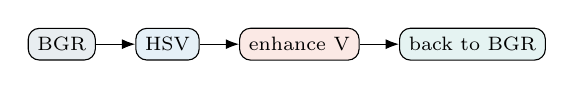
\begin{tikzpicture}[font=\scriptsize,node distance=5mm]
    \node[draw,rounded corners,fill=coursePrimary!10] (bgr) {BGR};
    \node[draw,rounded corners,fill=courseInfo!12,right=of bgr] (hsv) {HSV};
    \node[draw,rounded corners,fill=courseAccent!15,right=of hsv] (v) {enhance V};
    \node[draw,rounded corners,fill=courseGood!12,right=of v] (back) {back to BGR};
    \draw[-{Latex}] (bgr)--(hsv);\draw[-{Latex}] (hsv)--(v);\draw[-{Latex}] (v)--(back);
  \end{tikzpicture}
  \end{center}
\begin{lstlisting}[language=Python]
hsv = cv2.cvtColor(img, cv2.COLOR_BGR2HSV)
h, s, v = cv2.split(hsv)
v = cv2.createCLAHE(2.0, (8, 8)).apply(v)     # enhance value only
out = cv2.cvtColor(cv2.merge([h, s, v]), cv2.COLOR_HSV2BGR)
\end{lstlisting}
\end{frame}

% ==================================================================
\section{In-class exercise}
% ==================================================================

\begin{frame}{\faPen~In-class exercise (10 min)}
  \begin{infobox}[Threshold a shadowed meter]
  \end{infobox}
  You have a meter photo with a diagonal shadow: the top-left is dark, the bottom-right is bright.
  \begin{enumerate}
    \item You run global Otsu and the top-left digits disappear into black. Why?
    \item You switch to adaptive with \code{blockSize=11} and get speckle everywhere. What do you change?
    \item Order these for this image: gamma, adaptive threshold, CLAHE. What runs first, and why?
  \end{enumerate}
\end{frame}

\begin{frame}{\faPen~Debrief}
  \begin{itemize}
    \item (1) One global $T$ can't fit both lighting zones; the dark side falls entirely below $T$.
    \item (2) \code{blockSize} too small tracks noise — raise it (e.g. 31) and/or raise \code{C}.
    \item (3) Enhance \term{first} (CLAHE/gamma to even out and lift contrast), \term{then} adaptive threshold.
  \end{itemize}
  \keyidea{Uneven light $\rightarrow$ local methods. Enhance before you binarize, never after.}
\end{frame}

% ==================================================================
\section{Putting it together}
% ==================================================================

\begin{frame}{The DocScan enhancement$\rightarrow$mask chain}
  \begin{center}
  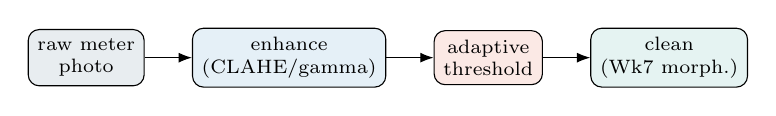
\begin{tikzpicture}[font=\scriptsize,node distance=6mm]
    \node[draw,rounded corners,align=center,fill=coursePrimary!10] (raw) {raw meter\\photo};
    \node[draw,rounded corners,align=center,fill=courseInfo!12,right=of raw] (enh) {enhance\\(CLAHE/gamma)};
    \node[draw,rounded corners,align=center,fill=courseAccent!15,right=of enh] (thr) {adaptive\\threshold};
    \node[draw,rounded corners,align=center,fill=courseGood!12,right=of thr] (clean) {clean\\(Wk7 morph.)};
    \draw[-{Latex}] (raw)--(enh);\draw[-{Latex}] (enh)--(thr);\draw[-{Latex}] (thr)--(clean);
  \end{tikzpicture}
  \end{center}
  \begin{itemize}
    \item Below $T$ vs above $T$ is a \term{classification} — errors here propagate to every later step.
    \item Too high $T$: digits break up. Too low: background bleeds in. Tune on \emph{hard} images.
    \item Each stage is deterministic and inspectable — save the intermediate images and look.
  \end{itemize}
\end{frame}

\begin{frame}{Thresholding is a decision, not a default}
  \begin{itemize}
    \item Choosing $T$ commits every pixel to one of two classes — there is no going back downstream.
    \item Global (Otsu) when lighting is even and the histogram is bimodal; adaptive when it isn't.
    \item Measure, don't guess: overlay the mask on the gray image and check the digit edges.
  \end{itemize}
  \begin{goodbox}
    Keep the enhancement deterministic and log the chosen $T$ — reproducibility beats a one-off pretty result.
  \end{goodbox}
\end{frame}

% ==================================================================
\section{Wrap-up}
% ==================================================================

\begin{frame}{What you should now be able to do}
  \begin{itemize}
    \item Threshold with a global (Otsu) or adaptive method, and know when each fails.
    \item Explain Otsu via between-class variance and compute it on a small histogram.
    \item Use CLAHE and histogram matching, and say why plain equalization can hurt a pipeline.
    \item Enhance color correctly (value channel, not per-RGB).
  \end{itemize}
\end{frame}

\begin{frame}{This week's deliverable}
  \begin{alertblock}{Due before Week 3 (see \code{project/})}
    On real meter/plate images from \code{E:/data}:
    \begin{enumerate}
      \item Plot the histogram; classify each image's exposure/contrast (from Session 1).
      \item Apply and compare: stretch, equalization, gamma, and CLAHE — with before/after.
      \item Produce a clean Otsu \emph{and} adaptive binary of the digits; say which wins and why.
      \item Note: for your DocScan image, which enhancement + threshold combo reads best?
    \end{enumerate}
  \end{alertblock}
\end{frame}

\begin{frame}[standout]
  Enhance for the goal, then commit with a threshold.\\[4pt]
  \normalsize A clean binary mask is what turns a meter photo into readable digits.
\end{frame}

\end{document}
